\documentclass[10pt,a4paper]{article}
\usepackage[margin=1.8cm]{geometry}
\usepackage{amsmath,amssymb}
\usepackage{booktabs}
\usepackage{tikz}
\usetikzlibrary{arrows.meta,positioning}
\usepackage[font=small]{caption}
\usepackage{titlesec}
\titlespacing*{\section}{0pt}{8pt}{3pt}
\setlength{\parindent}{0pt}
\setlength{\parskip}{3pt}
\allowdisplaybreaks

\newcommand{\code}[1]{\texttt{\small #1}}

\title{\vspace{-1.2cm}PATRONUS --- VTOL take-off dynamics\\[2pt]
\large Equations of \code{vtolto\_forces\_3GDL} and \code{vtolto\_dynamics\_3GDL} (2Wings, 3-DOF longitudinal)}
\author{}
\date{\vspace{-1.2cm}}

\begin{document}
\maketitle

\section{Overview}

The take-off is a 3-DOF longitudinal model evaluated at every collocation node
(and Hermite--Simpson midpoint). \code{vtolto\_dynamics\_3GDL} receives the node values
$Z = (\mathbf{x}, \mathbf{u})$, calls \code{vtolto\_forces\_3GDL} for the resultant forces, pitching moment and
rotor power, and returns the state derivatives. The same forces are reused by the path constraints
(\code{vtolto\_path\_constraints\_3GDL}). Forces are written in \emph{inertial axes} ($x$ forward, $h$ up),
so the model stays defined in hover, where the wind axes are not.

\begin{center}
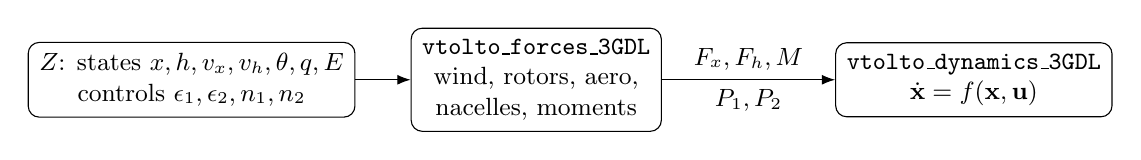
\begin{tikzpicture}[node distance=7mm, every node/.style={font=\small},
  box/.style={draw, rounded corners, align=center, inner sep=4pt, minimum height=9mm}]
\node[box] (z) {$Z$: states $x,h,v_x,v_h,\theta,q,E$\\controls $\epsilon_1,\epsilon_2,n_1,n_2$};
\node[box, right=of z] (f) {\code{vtolto\_forces\_3GDL}\\wind, rotors, aero,\\nacelles, moments};
\node[box, right=22mm of f] (d) {\code{vtolto\_dynamics\_3GDL}\\$\dot{\mathbf{x}} = f(\mathbf{x},\mathbf{u})$};
\draw[-{Latex}] (z) -- (f);
\draw[-{Latex}] (f) -- node[above]{$F_x, F_h, M$} node[below]{$P_1, P_2$} (d);
\end{tikzpicture}
\end{center}

\begin{table}[h]
\centering\small
\caption{Symbols and their \code{params} fields.}
\begin{tabular}{@{}llll@{}}
\toprule
Symbol & Field & Symbol & Field \\
\midrule
$m$, $I_{yy}$ & \code{mass}, \code{Iyy} & $S_w$, $S_t$, $S_f$ & \code{wing\_area}, \code{tailwing\_area}, \code{fus\_area} \\
$\rho$, $g$ & \code{rho}, \code{g} & $\bar c$, $\ell_f$ & \code{geo.c\_wing}, \code{fus\_Lref} \\
$D$, $N_e$ & \code{prop.diameter}, \code{prop.num\_engines} & $A_n$ & \code{prop.nacelle\_area} (one engine) \\
$\eta$ & \code{prop.eff} & $V_\varepsilon$ & \code{V\_eps} (hover regularisation) \\
$x_w, z_w$ & \code{geo.xw}, \code{geo.zw} & $x_t, z_t$ & \code{geo.xtw}, \code{geo.ztw} \\
$x_f, z_f$ & \code{geo.xfus}, \code{geo.zfus} & & \\
\bottomrule
\end{tabular}
\end{table}

Index $i\in\{1,2\}$ denotes the rotor group: group 1 at the wing (front), group 2 at the tail (rear),
each with $N_e$ engines. Aerodynamic and propulsive coefficients
($C_L, C_D, C_M, C_T, C_P, C_H, C_{D,n}$) are CasADi lookups selected in \code{models\_config}.

\section{Relative wind and angles}

The airspeed is regularised with $V_\varepsilon$ so that every expression is smooth at hover:
\begin{gather}
V = \sqrt{v_x^2 + v_h^2 + V_\varepsilon^2}, \qquad \cos\gamma = \frac{v_x}{V}, \qquad \sin\gamma = \frac{v_h}{V}, \\
u_b = v_x\cos\theta + v_h\sin\theta, \qquad w_b = v_x\sin\theta - v_h\cos\theta, \\
\alpha = \operatorname{atan2}\!\Big(w_b,\ \sqrt{u_b^2 + V_\varepsilon^2}\Big), \qquad \gamma = \theta - \alpha, \qquad
\xi = \xi_0 + \frac{\partial \xi}{\partial \alpha}\,\alpha \quad (\code{downwash\_calc}).
\end{gather}
$\alpha \to -90^\circ$ in a vertical climb and $\alpha=0$ in perfect hover; the formula assumes $u_b \ge 0$ (no backwards flight).
Rotor inflow angle and advance ratio:
\begin{equation}
\phi_i = \alpha + \epsilon_i, \qquad J_i = \frac{V}{n_i D}.
\end{equation}

\section{Rotor forces and power}

\begin{equation}
T_i = N_e\, C_T(J_i,\phi_i)\, \rho\, n_i^2 D^4, \qquad
H_i = N_e\, C_H(J_i,\phi_i)\, \rho\, n_i^2 D^4, \qquad
P_i = N_e\, C_P(J_i,\phi_i)\, \rho\, n_i^3 D^5 .
\end{equation}
$T_i$ acts along the rotor axis, at angle $\theta+\epsilon_i$ from the horizon; $H_i$ is normal to it.

\section{Aerodynamic forces (wind axes)}

With $\bar q = \tfrac12 \rho V^2$ and the tail seeing the downwash-reduced angle $\alpha - \xi$:
\begin{gather}
L_w = \bar q S_w C_{L,w}(\alpha), \quad D_w = \bar q S_w C_{D,w}(\alpha), \qquad
L_f = \bar q S_f C_{L,f}(\alpha), \quad D_f = \bar q S_f C_{D,f}(\alpha), \\
L_t' = \bar q S_t C_{L,t}(\alpha-\xi), \quad D_t' = \bar q S_t C_{D,t}(\alpha-\xi),
\end{gather}
and the tail forces rotated by the downwash into the freestream wind axes:
\begin{equation}
L_t = L_t'\cos\xi - D_t'\sin\xi, \qquad D_t = D_t'\cos\xi + L_t'\sin\xi, \qquad
L_a = L_w + L_f + L_t, \quad D_a = D_w + D_f + D_t .
\end{equation}

\section{Nacelle drag}

The induced velocity $v_i$ of each rotor group solves the momentum-theory quartic (the cruise model in
$\lambda = v_i/V$ multiplied through by $V^4$, so it stays finite at $V\to 0$):
\begin{equation}
v_i^4 + 2\sin\phi_i\, V v_i^3 + V^2 v_i^2 - K_i^2 = 0, \qquad K_i = \frac{T_i}{\tfrac12 \rho D^2},
\end{equation}
solved with 8 Newton iterations from the hover solution $v_i^{(0)} = \sqrt{K_i}$
(implemented as $(K_i^2 + 10^{-6})^{1/4}$):
\begin{equation}
v_i \leftarrow v_i - \frac{v_i^4 + 2\sin\phi_i V v_i^3 + V^2 v_i^2 - K_i^2}{4v_i^3 + 6\sin\phi_i V v_i^2 + 2V^2 v_i}.
\end{equation}
Local flow angle, dynamic pressure and drag at the nacelle:
\begin{gather}
\alpha_{n,i} = \operatorname{atan2}\!\big(V\sin\phi_i,\ v_i + V\cos\phi_i\big), \qquad
V_{n,i}^2 = V^2 + v_i^2 + 2\cos\phi_i\, v_i V, \\
D_{n,i} = C_{D,n}(\alpha_{n,i})\; \tfrac12\rho V_{n,i}^2\; A_n N_e .
\end{gather}

\section{Resultant force in inertial axes}

Aerodynamic forces are rotated from wind axes by $\gamma$; rotor forces act at $\theta+\epsilon_i$;
nacelle drag acts at $\theta+\epsilon_i-\alpha_{n,i}$ (opposing the local flow):
\begin{align}
F_x &= -D_a\cos\gamma - L_a\sin\gamma
 + \sum_{i=1}^{2}\Big[ T_i\cos(\theta+\epsilon_i) - H_i\sin(\theta+\epsilon_i) - D_{n,i}\cos(\theta+\epsilon_i-\alpha_{n,i}) \Big], \\
F_h &= -D_a\sin\gamma + L_a\cos\gamma
 + \sum_{i=1}^{2}\Big[ T_i\sin(\theta+\epsilon_i) + H_i\cos(\theta+\epsilon_i) - D_{n,i}\sin(\theta+\epsilon_i-\alpha_{n,i}) \Big] - m g .
\end{align}

\section{Pitching moment about the CG}

Pure aerodynamic moments of each surface (note the tail uses the wing reference area and chord, as in the code):
\begin{equation}
M_{A,w} = \bar q S_w \bar c\, C_{M,w}(\alpha), \qquad
M_{A,f} = \bar q S_f \ell_f\, C_{M,f}(\alpha), \qquad
M_{A,t} = \bar q S_w \bar c\, C_{M,t}(\alpha-\xi).
\end{equation}
Moments of the aerodynamic forces (positive nose-up):
\begin{align}
M_w &= L_w\cos\alpha\, x_w - L_w\sin\alpha\, z_w + D_w\sin\alpha\, x_w + D_w\cos\alpha\, z_w, \\
M_f &= L_f\cos\alpha\, x_f - L_f\sin\alpha\, z_f + D_f\sin\alpha\, x_f - D_f\cos\alpha\, z_f, \\
M_t &= -L_t\cos\alpha\, x_t - L_t\sin\alpha\, z_t - D_t\sin\alpha\, x_t + D_t\cos\alpha\, z_t .
\end{align}
Rotor moments (rotor 1 at $(x_w, z_t)$, rotor 2 at $(-x_t, z_t)$):
\begin{align}
M_{E,1} &= T_1\sin\epsilon_1\, x_w - T_1\cos\epsilon_1\, z_t + H_1\cos\epsilon_1\, x_w + H_1\sin\epsilon_1\, z_t, \\
M_{E,2} &= -T_2\sin\epsilon_2\, x_t - T_2\cos\epsilon_2\, z_t - H_2\cos\epsilon_2\, x_t + H_2\sin\epsilon_2\, z_t .
\end{align}
Nacelle drag moments:
\begin{align}
M_{n,1} &= D_{n,1}\sin(\epsilon_1-\alpha_{n,1})\, x_w + D_{n,1}\cos(\epsilon_1-\alpha_{n,1})\, z_w, \\
M_{n,2} &= -D_{n,2}\sin(\epsilon_2-\alpha_{n,2})\, x_t + D_{n,2}\cos(\epsilon_2-\alpha_{n,2})\, z_t .
\end{align}
Total:
\begin{equation}
M = M_{A,w} + M_{A,f} + M_{A,t} + M_w + M_f + M_t + M_{E,1} + M_{E,2} + M_{n,1} + M_{n,2}.
\end{equation}

\section{Equations of motion (\code{vtolto\_dynamics\_3GDL})}

\begin{equation}
\dot x = v_x, \qquad \dot h = v_h, \qquad
\dot v_x = \frac{F_x}{m}, \qquad \dot v_h = \frac{F_h}{m}, \qquad
\dot\theta = q, \qquad \dot q = \frac{M}{I_{yy}}, \qquad
\dot E = \frac{P_1 + P_2}{\eta}.
\end{equation}
$E$ is the battery energy consumed; the minimum-energy objective is $100\,E(t_f)/E_\text{batt}$.
These seven derivatives are what the collocation schemes (\code{collocation\_trapezoidal},
\code{collocation\_hermite\_simpson}) integrate, and $\dot v_x = \dot v_h = \dot q = 0$ at $t_f$ is the terminal trim condition.

\section{Alternative: body-axis (Stengel) formulation}

\emph{Not implemented; for comparison.} Stengel writes the longitudinal equations in body axes ($x_b$ forward,
$z_b$ down, $\theta$ nose-up) with the body velocity components $(u, w)$ as states:
\begin{equation}
X - mg\sin\theta = m(\dot u + q w), \qquad
Z + mg\cos\theta = m(\dot w - q u), \qquad
M = I_{yy}\,\dot q, \qquad \dot\theta = q,
\end{equation}
where $X$, $Z$ are the body-axis components of all forces except gravity, and $qw$, $-qu$ are the
transport terms of the rotating frame.

\textbf{States.} $u$ and $w$ are exactly the body velocities already used to compute $\alpha$ in Section~2:
\begin{gather}
u = v_x\cos\theta + v_h\sin\theta, \qquad w = v_x\sin\theta - v_h\cos\theta, \\
\dot x = v_x = u\cos\theta + w\sin\theta, \qquad \dot h = v_h = u\sin\theta - w\cos\theta . \label{eq:body_kin}
\end{gather}
The wind quantities then follow directly from the states:
$V = \sqrt{u^2 + w^2 + V_\varepsilon^2}$, $\alpha = \operatorname{atan2}(w, \sqrt{u^2 + V_\varepsilon^2})$, $\gamma = \theta - \alpha$.

\textbf{Body-axis forces.} With $z_b$ down, lift $\perp$ and drag $\parallel$ to the relative wind at angle $\alpha$, the rotor axis
at $\epsilon_i$ above $x_b$, and the nacelle drag opposing the local flow at $\epsilon_i - \alpha_{n,i}$:
\begin{align}
X &= -D_a\cos\alpha + L_a\sin\alpha
 + \sum_{i=1}^{2}\Big[ T_i\cos\epsilon_i - H_i\sin\epsilon_i - D_{n,i}\cos(\epsilon_i-\alpha_{n,i}) \Big], \\
Z &= -D_a\sin\alpha - L_a\cos\alpha
 + \sum_{i=1}^{2}\Big[ -T_i\sin\epsilon_i - H_i\cos\epsilon_i + D_{n,i}\sin(\epsilon_i-\alpha_{n,i}) \Big].
\end{align}
All force magnitudes ($L_a$, $D_a$, $T_i$, $H_i$, $D_{n,i}$) and the moment $M$ of Sections~3--7 are unchanged: they depend
on $\alpha$, $\epsilon_i$ and $V$, not on the axes used for the translational equations.
The $\theta$ dependence of the rotor and aerodynamic terms disappears from the forces and moves into the gravity
terms $mg\sin\theta$, $mg\cos\theta$.

\textbf{Equations of motion in body axes.}
\begin{gather}
\dot u = \frac{X}{m} - g\sin\theta - q w, \qquad
\dot w = \frac{Z}{m} + g\cos\theta + q u, \qquad
\dot q = \frac{M}{I_{yy}}, \qquad \dot\theta = q, \\
\dot x,\ \dot h \ \text{from \eqref{eq:body_kin}}, \qquad \dot E = \frac{P_1+P_2}{\eta}.
\end{gather}

\textbf{Equivalence with Section~8.} The non-gravity resultant rotates between frames as
$F_x = X\cos\theta + Z\sin\theta$ and $F_h + mg = X\sin\theta - Z\cos\theta$ (e.g.\ a rotor with
$X = T\cos\epsilon$, $Z = -T\sin\epsilon$ gives $F_x = T(\cos\epsilon\cos\theta - \sin\epsilon\sin\theta) = T\cos(\theta+\epsilon)$, as in Section~6).
Differentiating $u$ and $w$ and substituting $\dot v_x = F_x/m$, $\dot v_h = F_h/m$, $\dot\theta = q$:
\begin{align}
\dot u &= \dot v_x\cos\theta + \dot v_h\sin\theta + q\,(-v_x\sin\theta + v_h\cos\theta)
       = \frac{X - mg\sin\theta}{m} - q w, \\
\dot w &= \dot v_x\sin\theta - \dot v_h\cos\theta + q\,(v_x\cos\theta + v_h\sin\theta)
       = \frac{Z + mg\cos\theta}{m} + q u,
\end{align}
which are Stengel's equations. Both formulations describe the same dynamics; only the choice of
velocity states differs.

\textbf{What would change in the optimisation.}
\begin{itemize}\setlength{\itemsep}{1pt}
\item \emph{Bounds and boundary conditions.} Bounds on climb rate ($v_h \le 10$\,m/s) and forward flight ($v_x \ge 0$) are
box bounds in the inertial form but become nonlinear path constraints on $(u, w, \theta)$ in body axes;
conversely $u \ge 0$, the validity condition of the $\alpha$ formula, becomes a simple bound.
Hover conditions are unchanged: $v_x = v_h = 0 \Leftrightarrow u = w = 0$.
\item \emph{Terminal trim.} $\dot u = \dot w = \dot q = 0$ at $t_f$; with $u = w = q = 0$ there this is the same as
$\dot v_x = \dot v_h = 0$, i.e.\ $X = mg\sin\theta$, $Z = -mg\cos\theta$, $M = 0$.
\item \emph{Conditioning.} Body axes keep the aerodynamic forces a function of $(u,w)$ only and decouple them from
$\theta$, which is natural for wing-borne flight; inertial axes keep the translational equations linear in the
forces and free of the $q w$, $q u$ couplings, which suits hover and vertical climb. Large pitch rates make the
body-axis coupling terms more nonlinear for the collocation.
\end{itemize}

\section{Remarks}

\begin{itemize}\setlength{\itemsep}{1pt}
\item \textbf{Regularisation.} $V \ge V_\varepsilon > 0$ keeps $\cos\gamma$, $\sin\gamma$, $J_i$ and $\alpha$ smooth at hover;
aerodynamic forces scale with $V^2$ and vanish there, while nacelle drag does not ($v_i > 0$ in hover).
\item \textbf{Validity.} The $\alpha$ formula maps $|\alpha|<90^\circ$ and assumes $u_b \ge 0$; the bounds $x, v_x \ge 0$ enforce forward flight.
\item \textbf{Moment arms.} In $M_f$ the lift terms use arm $(x_f, z_f)$ but the drag terms imply $(x_f, -z_f)$, and the
nacelle drag arms ($M_{n,1}$ at $-x_w$, $M_{n,2}$ at $+x_t$ in the $r\times F$ sense) are opposite to their rotors. They are kept as in
\code{cruise\_constraints\_3GDL}.
\end{itemize}

\end{document}
